\documentclass[a4paper, 13pt]{article}
\usepackage[a4paper,top=50pt,bottom=50pt,left=30pt,right=30pt]{geometry}

\usepackage[french]{babel}

\usepackage{mathptmx}
\usepackage{enumitem}
\usepackage{graphicx}
\usepackage{longtable}

\newcommand{\q}[1]{``#1''}
\begin{document}
\title{Compte rendu de la séance 4}
\author{Ecaterina GUPCA, Alice MERAUD, Jean COSTREL DE CORAINVILLE, Romain REN et Faustin MILLET}
\maketitle

\section{Organigramme Technique}
\begin{figure}[h]
    \centering
    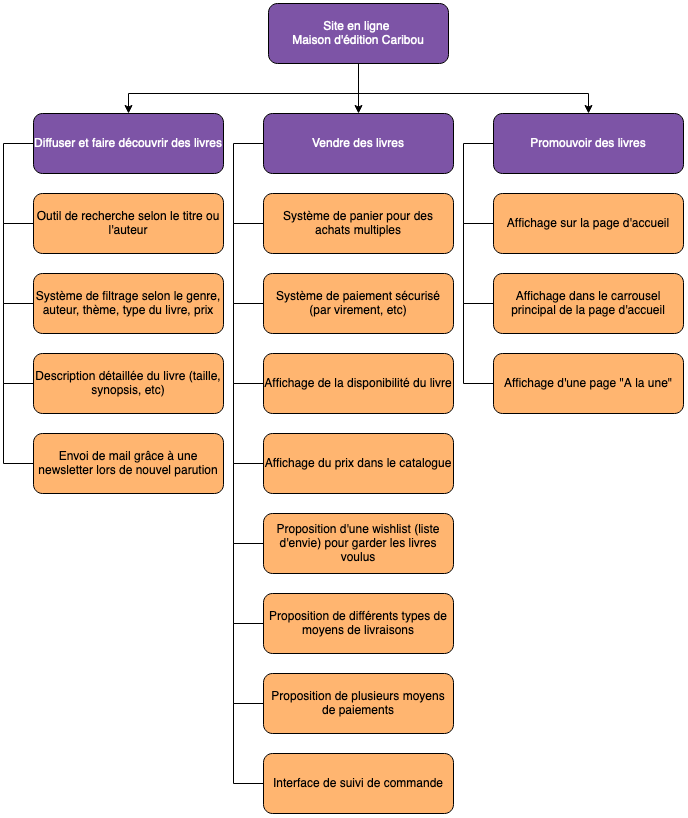
\includegraphics[width=0.8\linewidth]{images/diag_technique.png}
    \caption{Organigramme Technique}
\end{figure}
\section{jeux de données pour le test "achat d'un livre"}
\begin{center}
    \begin{longtable}{|c|c|c|c|c|}
        \hline
        \textbf{IdAuteur} & \textbf{NomAuteur} & \textbf{PrénomAuteur} & \textbf{EmailAuteur} & \textbf{TelAuteur} \\
        \hline
        \hline
        1 & Musso & Guillaume & \texttt{guillaume.musso@gmail.com} & 0607080910 \\
        2 & Dahl & Roald & \texttt{roald.dahl@folio.fr} & 0321495043 \\
        \hline
        \caption{Jeu de données pour la table Auteur}
    \end{longtable}
\end{center}
\begin{center}
    \begin{longtable}{|c|c|}
        \hline
        \textbf{IdGenre} & \textbf{NomGenre} \\
        \hline
        \hline
        1 & Aventure \\
        2 & Fantastique \\
        3 & Documentaire \\
        4 & Jeunesse \\
        \hline
        \caption{Jeu de données pour la table Genre}
    \end{longtable}
\end{center}
\begin{center}
    \footnotesize
    \begin{longtable}{|c|c|c|c|c|c|c|c|c|}
        \hline
        \textbf{IdLivre} & \textbf{ISBNLivre} & \textbf{TitreLivre} & \textbf{PrixLivre} & \textbf{DateParutionLivre} & \textbf{ExtraitPDFLivre} & \textbf{EnStockLivre} & \textbf{MiseEnAvantLivre} & \textbf{TailleLivre} \\
        \hline
        \hline
        1 & \texttt{2702183689} & Angélique & 21,90€ & 20/09/2022 & caribou.fr/1.pdf & true & true & 15.5 x 22.5 cm \\
        2 & \texttt{2070601595} & Angélique & 9,30€ & 16/06/2016 & caribou.fr/2.pdf & true & false & 12.5 x 18 cm \\
        \hline
        \caption{Jeu de données pour la table Livre}
    \end{longtable}
\end{center}
\begin{center}
    \begin{longtable}{|c|c|c|c|}
        \hline
        \textbf{IdClient} & \textbf{NomClient} & \textbf{EmailClient} & \textbf{MotdepasseClient} \\
        \hline
        \hline
        1 & Dupond & Paul & \texttt{Paul123} \\
        2 & Dupond & Miche & \texttt{Michel01} \\
        \hline
        \caption{Jeu de données pour la table Utilisateur}
    \end{longtable}
\end{center}
\begin{center}
    \begin{longtable}{|c|c|c|c|c|}
        \hline
        \textbf{IdAdresse} & \textbf{NuméroAdresse} & \textbf{NomAdresse} & \textbf{ComplémentAdresse} & \textbf{TéléphoneAdresse} \\
        \hline
        \hline
        1 & 5 & Rue des oliviers & Chambre 201 & null \\
        1 & 14 & Avenue des toiries & null & 0635442100 \\
        \hline
        \caption{Jeu de données pour la table Adresse}
    \end{longtable}
\end{center}
\begin{center}
    \begin{longtable}{|c|c|c|}
        \hline
        \textbf{IdGroupe} & \textbf{NomGroupe} & \textbf{PermissionGroupe} \\
        \hline
        \hline
        1 & Administrateur & 11111 \\
        1 & Commercial & 10101 \\
        1 & Auteur & 01101 \\
        1 & Libraire & 00111 \\
        1 & Client & 0011 \\
        \hline
        \caption{Jeu de données pour la table Groupe}
    \end{longtable}
\end{center}

\begin{center}
    \begin{longtable}{|c|c|c|c|}
        \hline
        \textbf{IdEntreprise} & \textbf{SIRETEntreprise} & \textbf{NomEntreprise} & \textbf{RemiseEntreprise} \\
        \hline
        \hline
        1 & \texttt{42324738600042} & Lagiraf & 25 \\
        2 & \texttt{50393256800010} & Carrefour & 22 \\
        3 & \texttt{42324738600042} & Lagiraf & 25 \\
        \hline
        \caption{Jeu de données pour la table Entreprise}
    \end{longtable}
\end{center}

\section{Scénario de test}
Pour essayer et vérifier ce cahier des charges, on peut tester différents scénarios d'essais.

\bigskip\noindent
\textbf{Si le client n'est pas inscrit}
\begin{itemize}
    \item Choisir un livre grâce aux outils de recherche et filtrer par les genres, titres ou auteurs
    \item Passer la commande dans le panier
    \item Vérifier qu'elle reste enregistrée dans le navigateur
    \item Retirer des livres du panier
    \item Remettre un livre différent
    \item Ajouter le même livre numérique et papier
    \item Passer la commande dans le panier et choisir le moyen de livraison
\end{itemize}
\bigskip
\textbf{Si le client est inscrit}
\begin{itemize}
    \item Ajouter un livre à la liste de souhaits
    \item Retirer ce livre de la liste de souhaits
    \item Se déconnecter
    \item Se reconnecter
    \item Vérifier que les livres sont toujours présents
    \item Passer la commande du livre
\end{itemize}
\end{document}   